After the thorough requirement analysis in Section \ref{sec::RequirementAnalysis} on which a concept for the software was derived in \ref{sec::Concept}, 
the following section will focus the implementation of the system components, starting with with the work- and interaction flow of the system.
Later, available commands and the concrete implementation details of surgical procedures and visualization tools will be discussed.
Lastly, architectural components as well as utilities provided by SteamVR will be shortly described.

%Architecture
As this thesis aims to offer an open-source framework for VR surgery, the most obvious choice for hardware was used.
A combination of commercially available HMDs and open source software is used to develop an easily accessible framework.
For this thesis, the VR HMD HTC Vive (Referenz later: $https://en.wikipedia.org/wiki/HTC_Vive$) together with the recent Valve Index Controller (Referenz later: $https://www.valvesoftware.com/en/index/controllers$) were used.
However, any commercially available headset and controller which is compatible with SteamVR will work with this system.
OpenVR (Referenz: https://github.com/ValveSoftware/openvr), the from Steam developed open-source Framework for VR development abstracts the HMD and specifics of controllers for the end user.
This way, even though we used a specific HMD and controller configuration for this thesis, any HMD and controller will work.

Since running virtual reality software is computationally expensive, a desktop pc with the following hardware is recommended for highest immersion:

\begin{compactenum}[label=(\alph*)]
    \item Graphics Card: Nvidia GTX 1060 or equivalent
    \item CPU: Intel i5-4590 / AMD Ryzen5 1500X
    \item Memory (RAM): 8GB+
\end{compactenum}

%SteamVR
The VR software was developed using Unity3D (LTS 2018.4), which is broadly accepted by the community and seen as an easy to learn tool (Referenz aus dem internet).
Inside of Unity, the OpenVR Toolkit provided by Steam and the included Teleportation system was used.
Additionally, SteamVRs interaction toolkit allows for natural hand interaction.
A realistic, and in the case of the Valve Index Controller real-time finger tracked representation of the users hands is projected into the VR.
It follows, that a natural interaction system where moving your hands to interact with the environment has been implemented.
Users interact with surgical instruments and the environment via their virtual hands.
A bare minimum of buttons was used to perform the procedures.
Solely the Graphical User Interface (GUI) and the execution of procedures is performed by pressing their respective button.

\section{\label{sec::Architecture}Architecture}

\begin{figure}[ht!]
    \centering
    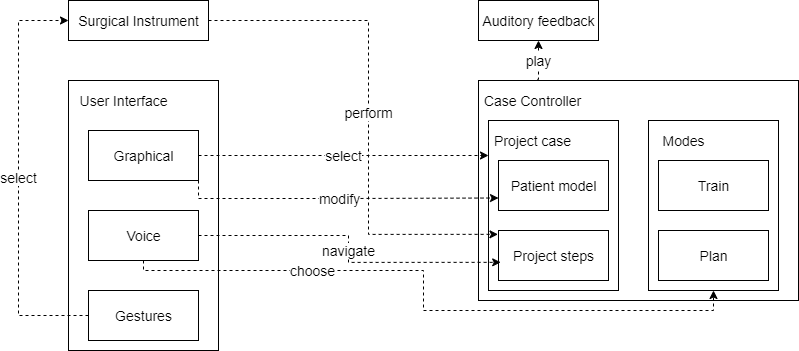
\includegraphics[width=\linewidth]{images/implementation/architecture.png}
    \caption{\label{fig::ImplementationArchitecture}High-level Overview of the Applications Architecture}
\end{figure}

The broad concept of the developed software is depicted in Figure \ref{fig::ImplementationArchitecture}.
The CaseController component is responsible for handling all project case related information.
Via the GUI, users load a project case into the CaseController.
Inside of the CaseController, users can choose to switch the currently active mode via the VUI.
The mode will decide how steps, which are added by the user via the currently selected surgical instrument, are handled inside of the CaseController.
In planning mode, steps are direkt added to the project case, while in training mode the correct exection of the procedure will be checked.
Either way, the CaseController calls the VoiceFeedback component to play auditory feedback to the user.
Surgical instruments are abstracted in such a way, that it does not matter which is currently selected for the CaseController.
New steps get passed to the CaseController in form of their 3D model with a new material attached to it.


\section{\label{sec::VitualOperatingRoom}Virtual Operating Room}
The increase the immersion of the VR, a virtual operating room has been designed with photogrammetry.
The virtual operating room has been modeled with a cost-effective, simplistic photogrammatry-esque approach, in which a real operation room from UHA has been captured using a 360 degree camera (Figure \ref{fig::360OperatingRoom}), the samsung gear 360, and converted into a 3D model via Walkabout Worlds (Referenz später: https://www.walkaboutworlds.com/).
For reference, the operating room 10 from UHA Aachen has been caputured and modeled after in VR.
Beforehand, the operating room was emptied out as much as possible and then after converting it to a 3D model filled with 3D object from open assets in Unity.
Some details, such as the operting table dock in the middle of the room and computer equiments have been edited out with photo-editing software.
The surgical instruments were scanned via medical imaging acquisition and postprocessed in Blender3D to reduce artifacts, which occur during the 3d scanning phase of the surgical instruments and materials.
After these critical steps for performance and immersion (especially for the OMF surgeons of UHA) have been completed, instruments and materials are ready to be imported into Unity3D.
User navigate through the software via a combination of natural gestures, Graphical- and Voice-User-Interface as will be discussed extensively in the following Section \ref{sec::UserInterface}.

\begin{figure}
    \centering
    \begin{minipage}{.5\textwidth}
      \centering
      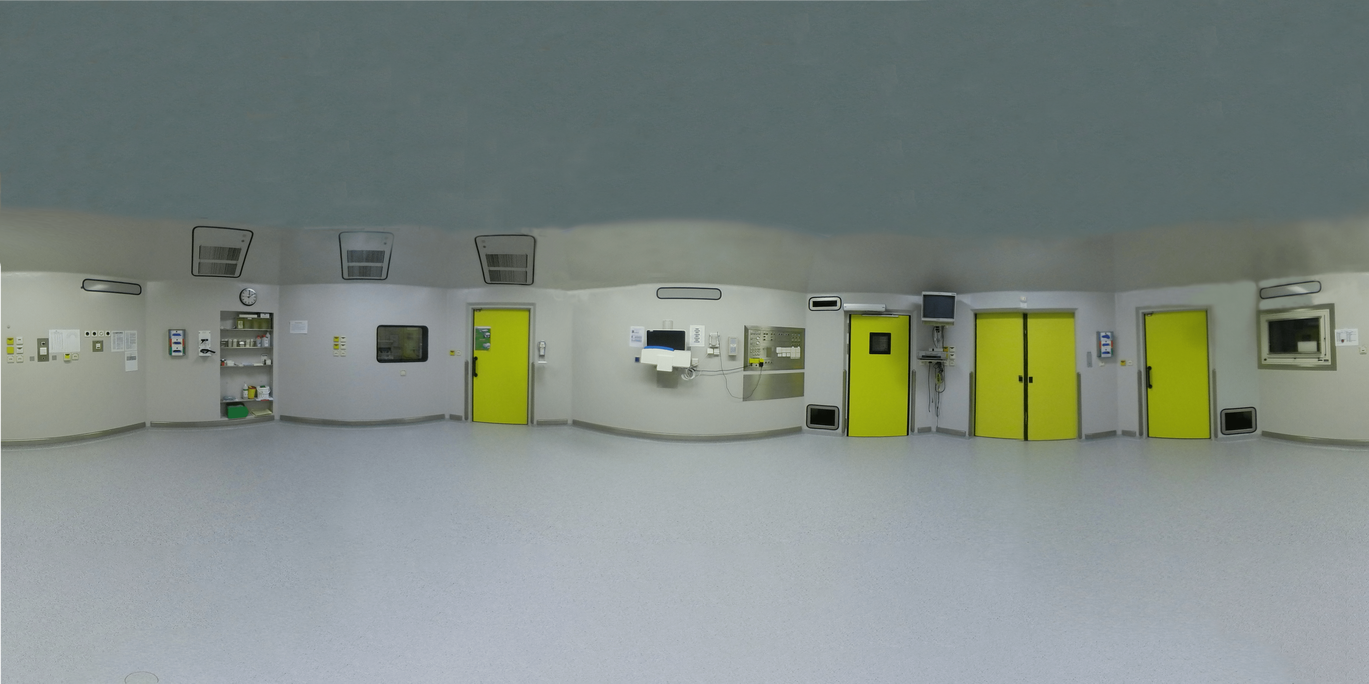
\includegraphics[width=0.95\linewidth]{images/implementation/operating_room_360.png}
    \end{minipage}%
    \begin{minipage}{.5\textwidth}
      \centering
      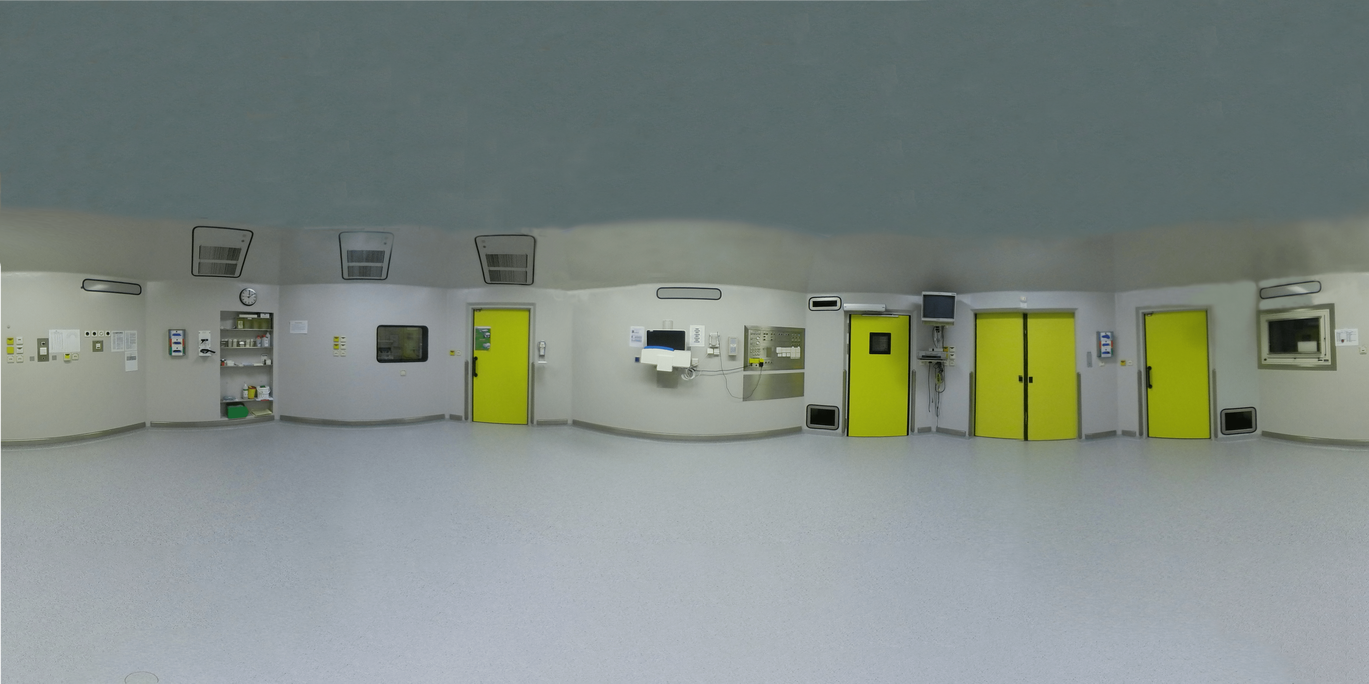
\includegraphics[width=0.95\linewidth]{images/implementation/operating_room_360.png}
    \end{minipage}
    \caption{\label{fig::360OperatingRoom}Left: Edited 360 Degree Photograph of OP 10 in UHA. Right: Result of conversion to 3D model via Walkabout Worlds}
\end{figure}